\chapter{Analysis}
\label{ch:analysis}

The concept for this thesis was to argue that breaking up the translation path from a formal specification to a full proof would be easier to conduct than to do a full proof all in one go. The vending machine example has been fully proved in \gls{ppz} and the birthday book example has been fully proved in \gls{hol}. We will now look at these to examples and compare them to the proofs done in a stepwise method using MathLang.

\section{Vending Machine Example}

The vending machine example shown in appendix \ref{app:vmspec} is a simple specification using only natural numbers as variables and there are no other types in the specification. 

\begin{table}[H]
\begin{center}
\begin{tabular}{| l || l | l | l | l |}
\hline
\textbf{Method} & \textbf{expertise} &  \textbf{input} & \textbf{lines of proof}  \\
& \textbf{required} & & \textbf{for first lemma (fl)}  \\
& & & \textbf{entire proof (ep)} \\
\hline
One step into & much & Either ascii or & fl = 19  \\
\gls{ppz} & & windows extended & ep = 140 \\
& & characters & (see appendix \ref{app:vm_ppz})\\
\hline
Multiple steps & little & \LaTeX{} partially & fl = 3  \\
using \gls{zmath} & & automated & ep = 124 (63 automated) \\
& & into Isabelle & (see appendix \ref{app:vm_mathlang}) \\
\hline
\end{tabular}
\end{center}
\caption{The vending machine proof using \gls{ppz} verses the \gls{zmath} proof.}
\label{tab:comparevm}
\end{table}

Table \ref{tab:comparevm} shows an outlined comparison between the vending machine proof done in \gls{ppz} (see appendix \ref{app:vm_ppz}) and the vending machine proof done using the \gls{zmath} method (see appendix \ref{app:vm_mathlang}). To calculate the lines of proof, all comments and empty lines have been removed from the proof and only the content is left. Although the syntax of the proof can differ depending on the author, for example some of the tactics can be put on a single line or can be put on two separate ones, the lines of proof give a rough estimate in the size of  proof.

Although the entire proof using the \gls{zmath} method is 124 lines, 63 of those lines are automatically generated using the annotated \LaTeX{} document (see \ref{app:vm_annotate}), which is 79 lines. This means that 50.8\% of the proof is already automatically generated without the user having any knowledge of the theorem prover they are using. The actual amount of lines in both the proofs are somewhat similar (140 lines compared with 124).

\begin{table}[H]
\begin{center}
\begin{tabular}{| l | l | l |}
\hline
\textbf{Type of} & \textbf{one step} & \textbf{multi step} \\
\textbf{expertise needed} & \textbf{into \gls{ppz}} & \textbf{using \gls{zmath}} \\
\hline
\hline
Knowledge of Z &  yes & yes \\
\hline
Knowledge of theorem prover & much & little \\
\hline
Knowledge of \LaTeX & some & yes \\
(including Z symbols) & (optional) & \\
\hline
Knowledge of how to & & \\
input specification into & yes & no \\
theorem prover & & \\
\hline
\end{tabular}
\end{center}
\caption{Expertise needed for one step proof in \gls{ppz} and multi step proof using \gls{zmath}.}
\label{tab:expertise}
\end{table}

The expertise needed to do either proof is shown in table \ref{tab:expertise}. Here we explain the different types of expertise needed in order to get the vending machine specification into a full proof using one step or using many steps.

\subsection{Knowledge of Z}
For both methods the user will need to have some form of Z specification knowledge. Using the \gls{zmath} method, the user also annotates the plain specification which would then in turn allow others (such as staff in the project team, software developers, etc) also understand the Z specification. Both methods need the same amount of expertise in Z and the \gls{zmath} method even shares some of the expertise with others looking at the documents produced.

\subsection{Knowledge of theorem prover}
In table \ref{tab:expertise}, it states that a "little" amount of knowledge of theorem prover is needed for the full proof using \gls{zmath}. This is because the final step is to prove any lemmas that are left unproven (these lemmas have been created from the original Z specification) and write new properties as lemmas and prove them if needed. However the original specification is automatically translated into your chosen theorem prover syntax and thus if the user needs to add more parts to the specification they already have an idea of the syntax to use. By translating the specification and proving it in one big step the user will need to learn how to input the specification first, as well the syntax of a specification in the chosen theorem prover language and write up a full proof. 

\subsection{Knowledge of \LaTeX}
The translation path using the \gls{zmath} methods assumes the user already knows how to write a Z specification using \LaTeX{}. The user then annotates these specifications using the annotations in the \gls{zmath} style package. The \LaTeX{} expertise required for the translation is enough so the whole Z specification is covered. The input of the schema boxes, Z characters etc are all imputed using the zed style package, which the user can learn using Mike Spivey's reference card \cite{zrefcard}.

The schema boxes and symbols are written in \gls{ppz}'s own syntax. \gls{ppz} also has a user interface, (PPXPP), in which it uses an extended character set instead of ascii to input the specifications and their proofs. In this, the user may open a palette in which they can search for the symbol they wish to use and click on it. The same works with schema boxes, axiomatic definitions, generic definitions etc. 

The translation method using \gls{ppz} requires some \LaTeX{} knowledge which is optional. This is only if the user wishes to extract the formal material for typesetting their proofs. The shell script \textbf{doctex} allows the user to prepare a \LaTeX{} file using the \gls{ppz} extended character set. However to typeset the proof the instructions say that some familiarity with \LaTeX{} is required.

\subsection{Knowledge of input of specification}
Discounting the tactics and lemmas needed to prove the specification. A large part of full proof for the specification is to input the specification itself into the chosen theorem prover. By translating the specification in one big step using \gls{ppz} the user must already have vast knowledge of \gls{ppz} to do this. That is, to translate the specification itself in one big step into \textbf{any} theorem prover requires a lot of knowledge about the chosen theorem prover. By using the \gls{zmath} method to translate the specification itself requires no knowledge about Isabelle by the user, as all the Isabelle syntax is automatically translated from the annotated specification written in \LaTeX{}. 

\section{Birthday Book Example}

The birthday book example (shown in appendix \ref{app:bbspec}), was created by Spivey \cite{spiveyreferencemanual}. This example is a specification which describes a system of a birthday book where the main functions include adding a person and their birthday, removing a person and their birthday etc. This system uses sets and it's own types, \texttt{NAME} and \texttt{DATE}.

\begin{table}[H]
\begin{center}
\begin{tabular}{| l || l | l | l | l |}
\hline
\textbf{Method} & \textbf{expertise} &  \textbf{input} & \textbf{lines of proof}  \\
& \textbf{required} & & \textbf{for first lemma (fl)}  \\
& & & \textbf{entire proof (ep)} \\
\hline
 \gls{hol} & some  & automated into  & fl = 5  \\
 & & ZeTa, manually into & ep = 361 \\
& & \gls{hol} & \\
\hline
 Multiple steps &  little & \LaTeX{} partially  & fl = 8  \\
using \gls{zmath} & & automated & ep = 120 \\
&  & into Isabelle &  \\
\hline
\end{tabular}
\end{center}
\caption{The birthday book proof using \gls{hol} verses the \gls{zmath} proof.}
\label{tab:comparebb}
\end{table}

Table \ref{tab:comparebb} shows the comparison between the birthday book proof done in \gls{hol} (see appendix \ref{app:bb_hol}) and the birthday book proof done using the \gls{zmath} method (see appendix \ref{app:bb_fullproof}). Again to calculate the lines of proof, all comments and empty lines have been removed from the proof. Since the birthday book proof in \gls{hol} comes in many different files, all the lines from these files have been added.

The first lemma (fl) in the table has been calculated from the "pre addBirthday lemma" which is called \texttt{lemma AddBirthdayIsHonest} in the \gls{zmath} method and \texttt{zlemma lemma2} in the \emph{Rel\_Refinement.thy} file using the \gls{hol} method. The full proof using the \gls{hol} method is 361 lines, however this is split up into 5 files. The \emph{BBSpec.holz} which is automatically generated using the ZeTa-to-\gls{hol} converter. This converted consists an adapter that is plugged into ZeTa and converts the \LaTeX{} specification into an SML-file. The \emph{BB.thy} file which is used to import \emph{Fun\_Refinement.thy} and \emph{Rel\_Refinement.thy} and \emph{BBSpec.thy} which is used to import the specification from the SML-file. In order to prove the specifications in \gls{hol}, there are 17 other theory files which have been created in order to use tactics an lemmas, these include \emph{ZSeq.thy}, \emph{Z.thy}, \emph{ZPure.thy}.

The raw \LaTeX{} file used for the \gls{hol} method is 97 lines (see appendix \ref{app:bb_annotate_hol}), this is automatically generated into an SML file which can be imported into \gls{hol} which is 17 lines long. The raw \LaTeX{} file which is used for the \gls{zmath} method is 96 lines (see appendix \ref{app:bb_annotate}) which automatically generates a single theory file containing the environment and the specification, this file is 70 lines.

\begin{table}[H]
\begin{center}
\begin{tabular}{| l | l | l |}
\hline
\textbf{Type of} & \textbf{large steps} & \textbf{small steps} \\
\textbf{expertise needed} & \textbf{into \gls{hol}} & \textbf{using \gls{zmath}} \\
\hline
\hline
Knowledge of Z &  yes & yes \\
\hline
Knowledge of theorem prover & some & little \\
\hline
Knowledge of \LaTeX & yes & yes \\
\hline
Knowledge of how to & some & no \\
input specification into &(sml into \gls{hol})&  \\
theorem prover &  &  \\
\hline
\end{tabular}
\end{center}
\caption{Expertise needed for one step proof in \gls{ppz} and multi step proof using \gls{zmath}.}
\label{tab:expertisebb}
\end{table}

Table \ref{tab:expertisebb} shows the type and amount of expertise needed in order to get from a specification into a fully proof.

\subsection{Knowledge of Z}

For both methods the user will need to have some knowledge of Z specifications. This is because in both methods the initial step is to write the specification in \LaTeX{} for the system. However by using the \gls{zmath} method when annotating the Z specification in ZCGa, toe compiled documents outputs the weak types in different grammars. This then allows others to identify certain parts of the Z syntax. Therefore the knowledge of Z is exactly the same in both these methods.

\subsection{Knowledge of theorem prover}

Table \ref{tab:expertisebb} shows that by using the \gls{zmath} method `little' knowledge of theorem prover is needed. This is because the final step to prove any unproven lemmas and write and new safety properties and lemmas and prove them. For this the user may need some theorem prover knowledge to compete this final step. However the entire specification itself is already written in the chosen theorem prover (in our case Isabelle) and the user does not need to import any further definitions which are part of the original specification. However, by using \gls{hol} method the user will need `some' theorem prover knowledge. Although it is possible to ease the translation of the specification into \gls{hol} using ZeTa (see section \ref{knowledgeofinputforbb}), the user will need to have the \gls{hol} plugin knowledge as well as the original Isabelle/Hol Knowledge to do the proofs for the specification.

\subsection{Knowledge of \LaTeX}

In both methods the user will need to have the same amount of knowledge of \LaTeX{}. This is because in both cases, the user will need to input their specification using \LaTeX{}. The only difference in this aspect is that the user will need to annotate their specification using \gls{zmath} annotations (ZCGa and ZDRa) in the \gls{zmath} method or the user will need to annotate their specification using \gls{hol} annotations (proof obligations, zsections etc). In both cases the user will need to know how to import a package into \LaTeX{} and then read the instructions in either case on the annotations which need to be used.

\subsection{Knowledge of input of specification}
\label{knowledgeofinputforbb}

When translating Z specification into the \gls{hol} theorem prover there are two ways a user can do this. The first method for convenience, involves the user writing their specification in \LaTeX{}, using the \gls{hol} package to annotate their specification. Then the ZeTa-to-\gls{hol} plug-in type checks the specification and generates .holz files which can be imported by the user into the \gls{hol} theorem prover. The method is have the user write the specification directly into \gls{hol} circumventing ZeTa.
In both these methods the user would need at least some form of \gls{hol} prover knowledge. The latter would need more than the former. By using the ZeTa-to-\gls{hol} plug-in, the user can write their specification in \LaTeX{} format with the \gls{hol} annotations (very similar to \gls{zmath} method), however the user will need to know how to import the .holz files into the \gls{hol} theorem prover, unpack the schemas and values, and how to write and prove the properties. 

To input the specification into the chosen theorem prover using \gls{zmath} the user will need no theorm prover knowledge at all. This is because the annotated specification will be automatically translated into Isabelle/Hol when using the \gls{zmath} method. The program will automatically generate an `.thy' file which is a skeleton of the specification and then automatically fill in the specification using the information from the ZCGa annotations.

\section{Conclusion}

Even when teaching the syntax of Z in an academic setting, the \gls{zmath} aspects and programs can be used as helpful tools to help students understand the syntax of their formal specifications.
%
%
%\subsubsection{Specification Input}
%
%We compare the way the specification is imputed into the theorem prover. Also it may be interesting to see how many lines are needed for the first lemma. We could compare the entire proof however with additional comments and information needed for the proofs this may be more complicating to analyse.
%
%\begin{figure}[H]
%\begin{BVerbatim}[fontsize=\scriptsize, baseline=t]
%%EZ%%BH%%BH%%BH%%BH%%BH%%BH%%BH%%BH%%BH%%BH%
%%SZS%exact_cash%BH%%BH%%BH%%BH%%BH%%BH%%BH%
%%BV%	cash_tendered? :%bbN%
%%BT%%BH%%BH%%BH%%BH%%BH%%BH%%BH%%BH%%BH%%BH%
%%BV%	cash_tendered? = price
%%EZ%%BH%%BH%%BH%%BH%%BH%%BH%%BH%%BH%%BH%%BH%
%\end{BVerbatim}
%\begin{BVerbatim}[fontsize=\scriptsize, baseline=t]
%	definition exact_cash :: 
% 	"nat  \<Rightarrow> bool"
%	where 
%	"exact_cash cash_tendered  \<equiv> 
%	(cash_tendered = price)"
%\end{BVerbatim}
%\caption{The exact\_cash schema written in \gls{ppz} (left) and Isabelle (right).}
%\label{fig:exact_cash}
%\end{figure}
%
%The input for a \gls{ppz} proof can be either in ascii or an extended character set.
%The ascii character set is to input the schemas of a Z specification into a normal text editor. Figure \ref{fig:exact_cash} shows the same schema (\emph{exact\_cash}), written both \gls{ppz} and Isabelle syntax. Note that the schema written in \gls{ppz} is more similar to a normal drawing of a schema than the Isabelle version. However with the ascii version of the Z schema it is difficult to distinguish between the actual words of the schema and the actual schema frame itself.
%
%\begin{figure}[H]
% \begin{center}
% 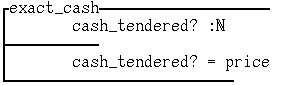
\includegraphics [width=6cm]{Figures/Conclusion/exactcash.png}
% \caption{The exact\_cash schema written in \gls{ppz} using the extended character set.}
% \label{fig:exactcash_ext}
%\end{center}
%\end{figure}
%
%On the other hand, when converting a \gls{ppz} proof into the extended character set. The Z specification is neater and shows the proper frames for the schema boxes. Figure \ref{fig:exactcash_ext} shows the exact\_cash schema box with the extended character set. However to get to this stage the user must first learn how to convert between the ascii and the extended character versions. They must also learn how to use the \textbf{xpp} interface \cite{xppMan}, which combines a general purpose editor with a command interface for the use of \gls{ppz}.
%
%\subsubsection{Expertise required in order to get a full proof}
%
%To actual obtain the full proof of the vending machine requires a lot less expertise if using the MathLang method than if going straight into a \gls{ppz} proof. Some knowledge about Z specifications may be required so that one may annotate what are declarations, expressions, state schemas etc. But no theorem prover knowledge is needed to actual insert the specification itself into Isabelle syntax (step 5 in figure \ref{fig:steps}). However to start writing the specification into \gls{ppz} the user will first need to read the \gls{ppz} manual to know how to get started. If using the ascii version they must know how to translate schema frames into ascii code and how to run the code. If using the extended character set, not only does the user need to learn \gls{ppz} syntax but also how to start and run the \textbf{Xpp} interface as well as the \gls{ppz} syntax. The user must also open the palette of symbols (which shows all symbols which can be used in Z) and search for the symbols needed.
%
%By using the \gls{zmath} steps as long as the user has labelled their specification correctly and checked it using ZCGa and ZDRa then the actual specification is automatically converted into Isabelle syntax. At no point during this translation does the user need to know or have used Isabelle previously. Nonetheless, from step 5 to step 7 the user will need to at least familiarise themselves with their chosen theorem prover (in this case Isabelle). Step 6 and step 7 include adding the properties the user wishes to prove as lemmas and then proving them. Since this is done in \gls{ppz} as well then this would be no extra effort then if the user has chosen to do it in one steps. But since the work from step 0 to step 5 is easier in steps using \gls{zmath} then the overall translation in \gls{zmath} would be easier to do.
%
%\subsubsection{Proof and tactics used to prove the lemma}
%
%\begin{figure}[H]
%\begin{BVerbatim}[fontsize=\scriptsize, baseline=t]
%set_goal([],%SZT%pre VM1 %equiv% 
%	(0 < stock
%	%and% cash_tendered? = price
%	%and% 0 %leq% takings)%>%);
%	
%a (rewrite_tac [VM1, VM_sale, some_stock,
% VM_operation, VMSTATE, exact_cash]);
%a (pure_rewrite_tac 
%[z_get_spec %SZT%(_ %leq% _)%>%]);
%a (rewrite_tac[]);
%a (REPEAT z_strip_tac);
%a (z_%exists%_tac %SZT%(
%	bars_delivered! %def% 1,
%	cash_refunded! %def% cash_tendered? 
%	+ ~ price,
%	stock' %def% stock + ~ 1,
%	takings' %def% takings + price)%>%
%   THEN rewrite_tac[]);
%a (PC_T1 "z_library_ext" asm_rewrite_tac
%   [rewrite_rule [] price]);
%a (LEMMA_T %SZT%stock + ~ 1 %leq% 
%stock%>% asm_tac THEN1 rewrite_tac[]);
%a (all_fc_tac [z_%leq%_trans_thm]);
%a (asm_rewrite_tac []);
%a (strip_asm_tac (z_get_spec %SZT%price%>%));
%a (all_fc_tac [z_%bbN%_plus_thm]);
%val pre_VM1_thm = save_pop_thm "pre_VM1_thm";
%\end{BVerbatim}
%\begin{BVerbatim}[fontsize=\scriptsize, baseline=t]
%lemma pre_VM1:
%"(\<exists> stock' takings' cash_refunded 
%bars_delivered.
% VM1 cash_tendered stock takings stock' takings' 
% cash_refunded bars_delivered)
% \<longleftrightarrow> (0 < stock) \<and> 
% (cash_tendered = price) \<and> (0 \<le> takings)"
% 
%apply (unfold VM1_def exact_cash_def some_stock_def
% VM_sale_def)
%apply auto
%done
%\end{BVerbatim}
%\caption{The exact\_cash schema written in \gls{ppz} (left) and Isabelle (right).}
%\label{fig:lemma1proof}
%\end{figure}
%
%We will now compare a lemma and it's proof inputted in both \gls{ppz} and Isabelle. Figure \ref{fig:lemma1proof} shows the same lemma and it's proof written in both \gls{ppz} (left) and Isabelle (right). The lemma and it's proof are both for the vending machine example. We can imagine that the vending machine specification is already in putted in the theorem prover before this lemma is added. We can see that the lemma itself is slightly longer written in Isabelle then it is in \gls{ppz}. However the proof of this lemma is a lot longer in \gls{ppz} then it is in Isablle. Note that at the end of the proof in \gls{ppz} we have the following line:
%\begin{verbatim}
%val pre_VM1_thm = save_pop_thm "pre_VM1_thm";.
%\end{verbatim}
%This saves the lemma and names it "pre\_VM1\_thm" whereas in Isabelle we have the lemma saved as "pre\_VM1" automatically. As this lemma and it's proof are part of step 6 and 7 of figure \ref{fig:steps} which are both manual input. It is both up to the user to acquire at least some knowledge of the targeted theorem prover in order to choose the lemmas and prove them. In this case writing the properties and proving them require the same amount of work in both scenarios, whether the user is proving the specification all at once or using the \gls{zmath} steps. However when using the \gls{zmath} path, steps 0 to 6 require less expertise knowledge.
%
%
%\subsection{Birthday Book Example}
%Spiveys birthday book is a specification which adds names and birthdays to a birthday book. It uses it's own types and sets.
%
%\begin{table}[H]
%\begin{center}
%\begin{tabular}{| l || l | l | l |}
%\hline
%\textbf{Method} & \textbf{expertise} &  \textbf{input}  \\
%& \textbf{required} &   \\
%\hline
%1 step into \gls{hol} & much & \LaTeX{} into    \\
%&  &  ZeTa into \gls{hol}   \\
%\hline
%stepwise using & little & \LaTeX{} into Isabelle    \\
%\gls{zmath} & &  \\
%\hline
%\end{tabular}
%\end{center}
%\caption{Comparison of the vending machine proof using \gls{ppz} Vs the \gls{zmath} method.}
%\label{tab:comparebb}
%\end{table}
%
%\subsubsection{Expertise required to get into a full proof}
%
%Similarly to \gls{zmath}, \gls{hol} breaks the translation into steps. It first reads a \LaTeX{} specification (again similar to \gls{zmath}), is type checked by ZeTa type checker and then is converted into SML-files that can be loaded in Isabelle. The SML files which are loaded into Isabelle need all the extra \gls{hol} .thy files to be checked, whereas \gls{zmath} only uses Isabelle's Main.thy package and nothing else. Therefore in order to prove the specification the user must learn all the extra \gls{hol} proving syntax as well as Isabelle's syntax and the Zeta type checker. Whereas in \gls{zmath} the user will only need to learn some Isabelle syntax in order to prove the properties of the specification.
%
%On the other hand \gls{hol} does have an advantage in that the by using the holz.sty package the user can use labels to automatically generate constancy conditions, refinement conditions or special safety properties. Thus, removing the effort from the user of doing these by hand.
%
%Since \gls{zmath} breaks the translation in more steps then \gls{hol}, it also has the advantage of being able to translate semi-formal specifications into theorem provers. Such that the specification can be written partially in Z format and partially in natural language. Another asset of the \gls{zmath} method is that the files produced from this method give not only the user but the programmers more information about the specification. By labelling the specification, the user is giving information about the types in the specification which can aid the developer in his work. The dependency graph and GoTo graph produced from the ZDRa also benefit the developers as they are then able to view the relationships between different parts of the specification. This will be especially beneficially on large scale projects where the different parts of the specification which relate to each other are far apart on the specification document.
%
%\subsubsection{Input}
%
%\begin{figure}[H]
%\begin{BVerbatim}[fontsize=\scriptsize, baseline=t]
%(ZAbsy.Eqn("AddBirthday", ZAbsy.SchemaText
%([ZAbsy.Unary(ZAbsy.Delta,ZAbsy.NameAppl
%("BirthdayBook",[])),ZAbsy.Direct
%(["name?"],ZAbsy.NameAppl("NAME",[])),
%ZAbsy.Direct(["date?"], ZAbsy.NameAppl
%("DATE",[]))],[ZAbsy.Test(ZAbsy.Tuple
%([ZAbsy.NameAppl("name?",[]),ZAbsy.
%NameAppl("known",[])]), ZAbsy.NameAppl
%("_notin_",[])),ZAbsy.Test(ZAbsy.Tuple
%([ZAbsy.NameAppl("birthday'",[]),ZAbsy.
%Binary(ZAbsy.Apply,ZAbsy.NameAppl
%("_cup_",[]),|Absy.Tuple([ZAbsy.NameAppl
%("birthday",[]),ZAbsy.Display([ZAbsy.
%Binary(ZAbsy.Apply,ZAbsy.NameAppl
%("_mapsto_",[]),ZAbsy.Tuple([ZAbsy.
%NameAppl("name?",[]),ZAbsy.NameAppl
%("date?",[])]))])]))]),ZAbsy.NameAppl
%("_=_",[]))]),ZAbsy.Type(ZAbsy.Unary(ZAbsy.
%Power,ZAbsy.Signature([("birthday",ZAbsy.
%Unary(ZAbsy.Power,ZAbsy.Product([ZAbsy.
%NameAppl("NAME",[]),ZAbsy.NameAppl("DATE",
%[])]))), ("birthday'",ZAbsy.Unary(ZAbsy.
%Power,ZAbsy.Product([ZAbsy.NameAppl("NAME",[])
%,ZAbsy.NameAppl("DATE",[])]))),("date?",
%ZAbsy.NameAppl("DATE",[]("known",ZAbsy.
%Unary(ZAbsy.Power,ZAbsy.NameAppl("NAME",[]))),
%("known'",ZAbsy.Unary(ZAbsy.Power,ZAbsy.
%NameAppl("NAME",[]))),("name?",ZAbsy.
%NameAppl("NAME",[]))]))))),
%\end{BVerbatim}
%\begin{BVerbatim}[fontsize=\scriptsize, baseline=t]
%definition AddBirthday :: 
%"BirthdayBook => BirthdayBook =>  NAME set => 
%(NAME * DATE) set => NAME => DATE => bool"
%where 
%"AddBirthday birthdaybook birthdaybook' known'
% birthday' name date ==
%(
%(name \<notin> known)
%\<and>
%(birthday' = birthday \<union> {(name, date)})
%)"
%\end{BVerbatim}
%\caption{The AddBirthday schema written in \gls{hol} (left), and \gls{zmath} (right).}
%\label{fig:addbirthdaydef}
%\end{figure}
%
%Figure \ref{fig:addbirthdaydef} shows the AddBirthday Schema from the birthday book automatically generated into \gls{hol} on the left and \gls{zmath} on the right. Although both of these are automatically generated and not user input, the input into Isabelle through \gls{zmath} would be a lot easier for anyone to understand. The \gls{hol} input is a separate theory  file and in the main .thy file has the line "load\_holz "BBSpec"" is added. The user may want to go through some functions and make changes to the original specification, to do this the user would need to go back to the \LaTeX{} specification and go through the process again, or learn the syntax of Isabelle and \gls{hol} in greater detail in order to add more functions.
%
